\documentclass{beamer}
% \usepackage{beamerthemesplit} // Activate for custom appearance
\usepackage{beamerthemesintef}

\titlebackground*{assets/background}
\title{Point Cloud Occupancy with Dynamic Planes}
\subtitle{Computer Vision Course Project}
\course{Master's Degree in Artificial Intelligence and Robotics}
\author{\href{mailto:bugli.1934824@studenti.uniroma1.it}{Eugenio Bugli}}
\IDnumber{1934824}
\date{Academic Year 2024/2025}

\begin{document}
\maketitle

\section{Introduction}

\begin{frame}{TODO}
\begin{itemize}
\item check UNet
\item reconstruction
\item bilinear interpolation
\item metrics
\item slides
\end{itemize}
\end{frame}

\begin{frame}{What is the Addressed Problem}
\begin{itemize}
	\item In this work we are interested in performing the reconstruction of point clouds. 
	\item The input noisy point clouds are encoded into per-point features that are projected onto multiple 2D dynamic planes.
	\item Then we predict the occupancy values of each point in order to find the surface of the shapes.
	\item The original paper applied this study to the ShapeNet Dataset.
\end{itemize}
\end{frame} 

\begin{frame}{Point Clouds, Meshes and Ground Truths}
Insert 3 images of the same sample
\end{frame}

\section{Dataset}

\begin{frame}{FAUST Dataset}
    This Dataset is composed by high-resolution human scans of 10 different bodies in 30 different poses. 
    \begin{itemize}
    \item The test set is composed by 200 scans, while the training has 100 scans.
    \item Each of the samples inside the training set has a corresponded ground truth alignment (registration)
    \item The training set has been partitioned again in order to obtain train and validation sets
    \item About 80 \% fo the initial training set has been used for training, while the other 20 \% has been used for validation 
    \end{itemize}
\end{frame}

\begin{frame}{Examples from the Dataset}
Insert here 1/2 images of different bodies with differente poses. Registration + Clouds
\end{frame}

\begin{frame}{Sampling}
    The perfomances of the Architecture varies with respect to the Sampling technique used. The author of the paper have used a Uniform Sampling, while in my case I have tried different approaches, each with different pros and cons:
    \begin{itemize}
    \item Random Sampling
    \item Importance Sampling
    \item Uniform Sampling
    \end{itemize}
\end{frame}

\begin{frame}{Examples of Sampled Clouds}
Insert here images of the sampled point cloud in the 3 Cases + Real cloud
\end{frame}

\section{Architecture}

\begin{frame}{Architecture design}
The Architecture is characterized by an Encoder-Decoder structure:
\begin{itemize}
\item Encode the input clouds into 2D Feature Planes
\item Decode these features into occupancy probabilities
\end{itemize}
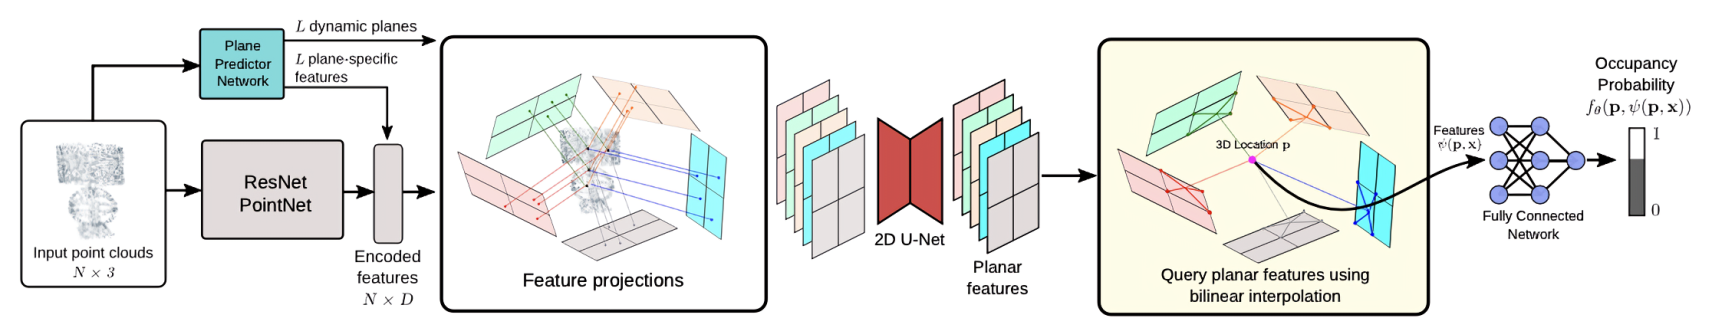
\includegraphics[width=\textwidth]{../media/architecture.png}
\end{frame}

\begin{frame}{Encoder}
The Encoder is composed by :
\begin{itemize}
\item ResNet PointNet
\item Plane Predictor 
\item UNet
\end{itemize}
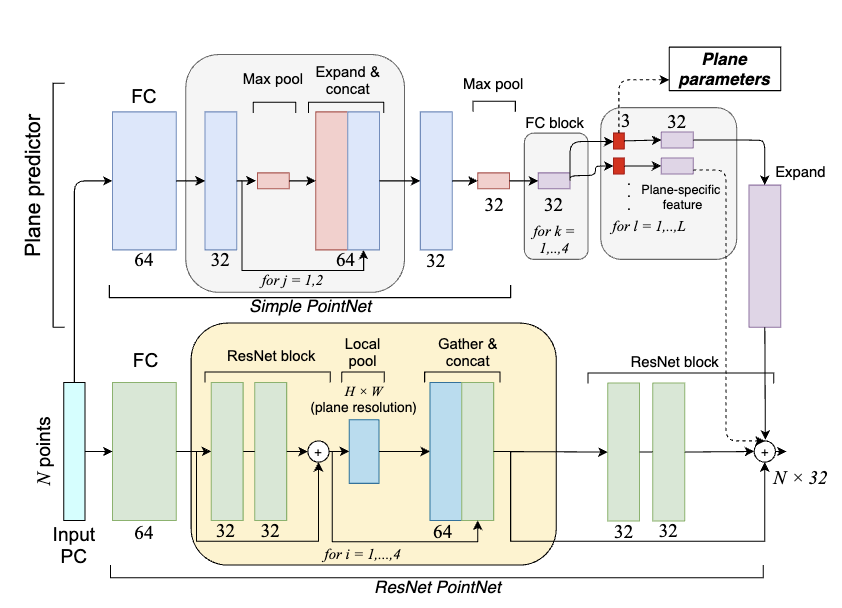
\includegraphics[width=\textwidth]{../media/encoder.png}
\end{frame}

\begin{frame}{Decoder}
The Dec is composed by:
\begin{itemize}
\item Feature Projection and Bilinear Interpolation
\item Occupancy Network
\end{itemize}
\end{frame}

\section{Reconstruction}

\begin{frame}{Reconstruction Phase}
\end{frame}

\section{Results}

\begin{frame}{Metrics}
In order to evaluate the performance of our model, the following metrics have been used:
\begin{itemize}
\item Chamfer Distance : \\ 
$
CD(A, B) = \frac{1}{|A|} \sum_{a \in A} \min_{b \in B} \|a - b\|_2^2 + \frac{1}{|B|} \sum_{b \in B} \min_{a \in A} \|b - a\|_2^2
$
\item IOU : 
$ IoU(A', B') = \frac{|A' \cap B'|}{|A' \cup B'|}$
\item F-Score:
\end{itemize}
Add each formula
\end{frame}

\begin{frame}{Loss Performances}
Insert here plots
\end{frame}

\begin{frame}{Metrics Performances}
Insert here just a table with metrics, gpu usage
various types of sampling
\end{frame}

\begin{frame}{ReconstructionPerformances}
Insert here just some images about reconstructions
\end{frame}

\section{Improvements}

\begin{frame}{Possible Changes and Future Improvements}
\end{frame}

\backmatter
\end{document}